% !TeX spellcheck = en_GB

\documentclass{beamer}

\usetheme{Warsaw}             % Falls Ihnen das Layout nicht gef�llt, k�nnen Sie hier
                              % auch andere Themes w�hlen. Ein Verzeichnis der m�glichen 
                              % Themes finden Sie im Kapitel 15 des beameruserguide.


\setbeamertemplate{footline}[frame number] %Seitenzahlen

\usepackage[utf8]{inputenc} % um Umlaute direkt eingeben zu
\usepackage[english]{babel}
\usepackage{amsmath}
\usepackage{amsfonts}
\usepackage{amssymb}
\usepackage{graphicx}
\usepackage{tikz}
\usepackage{stmaryrd} % for llbracket
\usepackage{algorithm} %for algorithms
\usepackage{algpseudocode} %for algorithms
%\usepackage{caption}
\usepackage{subcaption} %for subfigure
\usepackage[3D]{movie15} %for interactve 3d plot 

\usepackage{wrapfig} % for using wrapfigure

\usepackage{bigdelim}
\usepackage{caption}
\usepackage{subcaption}
\usepackage{ltxtable}
\usepackage{float}
%\usepackage{pgfplotstable, booktabs} %to generate tables from data files
\usepackage{cancel} %um durchzustreichen


\usepackage{bibunits} %to split bibliography

\usepackage{../Arbeit/makros}
\usepackage{todo}

\makeatletter
% Detect mode. mathpalette is used to detect the used math style
\newcommand<>\Alt[2]{%
    \begingroup
    \ifmmode
        \expandafter\mathpalette
        \expandafter\math@Alt
    \else
        \expandafter\make@Alt
    \fi
    {{#1}{#2}{#3}}%
    \endgroup
}

% Un-brace the second argument (required because \mathpalette reads the three arguments as one
\newcommand\math@Alt[2]{\math@@Alt{#1}#2}

% Set the two arguments in boxes. The math style is given by #1. \m@th sets \mathsurround to 0.
\newcommand\math@@Alt[3]{%
    \setbox\z@ \hbox{$\m@th #1{#2}$}%
    \setbox\@ne\hbox{$\m@th #1{#3}$}%
    \@Alt
}

% Un-brace the argument
\newcommand\make@Alt[1]{\make@@Alt#1}

% Set the two arguments into normal boxes
\newcommand\make@@Alt[2]{%
    \sbox\z@ {#1}%
    \sbox\@ne{#2}%
    \@Alt
}

% Place one of the two boxes using \rlap and place a \phantom box with the maximum of the two boxes
\newcommand\@Alt[1]{%
    \alt#1%
        {\rlap{\usebox0}}%
        {\rlap{\usebox1}}%
    \setbox\tw@\null
    \ht\tw@\ifnum\ht\z@>\ht\@ne\ht\z@\else\ht\@ne\fi
    \dp\tw@\ifnum\dp\z@>\dp\@ne\dp\z@\else\dp\@ne\fi
    \wd\tw@\ifnum\wd\z@>\wd\@ne\wd\z@\else\wd\@ne\fi
    \box\tw@
}

\makeatother



\AtBeginSection[]{\frame<beamer>{\frametitle{Content} \tableofcontents[current]}}

%\titlehead{\includegraphics[height=0.5cm]{../Arbeit/rwth.pdf} \hspace{1cm}
%\includegraphics[height=0.5cm]{../Arbeit/IGPM_logo_klein.png}
%}

\subject{Master Thesis}
\title{Discontinuous Galerkin Methods for the \MA Equation}
\subtitle{\Large Discontinuous Galerkin Verfahren zur Lösung der Monge-Amp\`ere-Gleichung}
\author{Elisa Friebel} %\\ Matrikelnummer: 295932
\date{\today}
%\publishers{Gutachter: Prof. Dr. rer. nat. W. Dahmen\\ Prof. Dr. rer. nat. S. Noelle}
\date{20. Januar 2015 \\[.5\baselineskip] Mastervortrag}

\begin{document}
\frame{\maketitle}

\begin{bibunit}[plain]

\section{\MA Equation}

\begin{frame}{The \MA Equation}
\begin{block}{\MA (MA) equation  with Dirichlet boundary data}
 \begin{align*}
	 \mydet{D^2 u} &= f \textnormal{ in } \Omega \\ %\label{eq: MA eq}\\
	 u & = g \textnormal{ on } \partial \Omega, %\label{eq: MA equation dirilecht} 
 \end{align*}
 \end{block}
\pause
Applications areas of equation of \MA type
\begin{itemize}
	\item astrophysics
	\item differential geometry
	\item finance
	\item optimal transportation 
	\item optics
\end{itemize} 
\end{frame}

%\subsection{Existence and Uniqueness}
\begin{frame}{Existence of solutions}
	Let $F$ be the \MA operator, i.e. $F= \detHess{u} - f$
	\begin{itemize}
		\item F is fully nonlinear second order operator
		\pause
		\item $F$ is elliptic for strictly convex functions $u$ and $f > 0$. %\cite{GT1983}
		\pause
		\item existence of a classical solution depends on the regularity of the data and domain
		\pause
		\item classical solutions are ambiguous
		\pause
		\item no general weak formulation \\
		 $\rightarrow $ in particular, no variational formulation
	\end{itemize}
\end{frame}

\begin{frame}{Weak Solution Notion}
	\begin{block}{Viscosity Solution{\cite[Definition 1.1]{FGN2013}}}
		We call a strictly convex $u \in C^0(\Omega)$ a \emph{viscosity subsolution (supersolution)} of the \MA equation, if for every point $x_0 \in \Omega$ and function $\varphi \in C^2(\Omega)$ satisfying
		\[
		   u \leq \varphi \;(\geq \varphi) \text{ in }\Omega \text{  and  } u(x_0) = \varphi(x_0)
		\]		there holds
		\[
			F[\varphi](x_0) \leq 0 \;(\geq 0).%\mydet{D^2 \varphi(x_0)} - f \leq 0 (\geq 0).
		\]

\end{block}
	Viscosity solutions are unique.
	%u-\varphi hat ein maximum(minimum), d.h. DF(u-\varphi)\leq(\geq)
\end{frame}

%\subsection{Numerical Schemes}
\begin{frame}{Numerical schemes}
They can roughly be divided into four categories \cite[p.210]{FGN2013}: 
\begin{enumerate}
	\item direct finite difference schemes,
	\item methods based on variational principles and approximating infinite-dimensional spaces by finite-dimensional spaces,
	\item methods based on finite basis expansions and approximating PDEs at sampling points,
	\item methods that do not fit in any of the three previous areas.
\end{enumerate}

\end{frame}

\begin{frame}{Finite difference schemes (FDS)}
Standard FDS (e.g. the nine-point stencil) 
are ambiguous:\\
	Solving the nonlinear system of equations Newton's method yields different results varying the initial guess 
\pause

Advantages of FDS
\begin{itemize}
	\item convergence proof template
	\item converge provably to viscosity solutions
\end{itemize}
\begin{columns}[c]
\begin{column}{0.55\textwidth}
\pause

Disadvantages of FDS
\begin{itemize}
	\item no proven convergence rates
	\item wide stencils, not applicable to many domains
	\item no nested iteration 
\end{itemize}
\end{column}

\pause
\begin{column}{0.35\textwidth}
\begin{figure}
  \begin{center}
    \input{stencil17.pgf}
  \end{center}
\end{figure}

\end{column}
\end{columns}
\end{frame}

\begin{frame}{Finite element methods (FEM)}
Advantages of FEM
\begin{itemize}
	\item expendable to complex domains
	\item good to parallelise
\end{itemize}
\pause
Disadvantages of FEM
\begin{itemize}
	\item no variational formulation
	\item there does not exist a FEM proven to converge to viscosity solutions
	\item nested iterations are easy to realise
\end{itemize}
\end{frame}

\section{A Discontinuous Galerkin Method for the \MA Equation}
\subsection{Motivation}
\begin{frame}{Picard linearisation}
\begin{itemize}
\item Convection term: $\nabla \cdot (A(u) \nabla u )$
\item Decoupling of the coefficient matrix $A(u)$ and $\nabla u$
\item One solves iteratively for $i\in \N$ the equations
	\begin{align}
	\nabla \cdot (A(u^{i} )\nabla u^{i+1}) \label{eq: Picard linearisation}
	\end{align}
\item \eqref{eq: Picard linearisation} is linear in $u^{i+1}$.
\item Converges slower than Newton's method, but has a larger convergence radius
\end{itemize}
\end{frame}

\begin{frame}{Decoupling of the MA equation}
\begin{align*}
\visible<1->{	
	&\dyy u{x}  \dyy u{y}  -\dyx u {x}{y} \dyx u {y}{x} = f} \\
	\visible<2->{\Leftrightarrow \; &\mycof {D^2 u }:D^2 u  = 2f,}
\end{align*}
\visible<2->{where in the two-dimensional case the cofactor matrix of $D^2 u$ is defined by
\[
	\cofHess u := \begin{pmatrix}
		u_{xx} & - u_{xy} \\
		-u_{yx} & - u_{yy} 
	\end{pmatrix}.
\]}
\visible<3->{
Divergence form
\begin{align*}
	- \nabla \cdot \left( \mycof{ D^2 u} \nabla u \right)  = -2f. 
\end{align*}
}
\end{frame}

\begin{frame}{Picard iteration to solve the MA equation}
	Given an initial guess $u^0$ solve for $i \in \N$
	\begin{align}
		- \nabla \cdot \left( \cofHessH{u^i} \nabla u^{i+1} \right)  = -2f \label{eq: Picard Iteration}
	\end{align}
	\pause via the symmetric interior penalty Galerkin (SIPG) method.

	\pause
	\begin{itemize}
		\item \eqref{eq: Picard Iteration} is a generalised Poisson problem (GPP)\\
			\pause $\rightarrow$ i.e. linear in the second derivatives of $u_h^{n+1}$
		\item discontinuous elements because $\cofHessH{u_h^n}$ is discontinuous (for standard finite elements)
	\end{itemize}

\end{frame}

\subsection{Symmetric Interior Penalty Galerkin}

\begin{frame}{Discrete variational formulation of the GPP}
Assume a triangulation $\triang$ of $\Omega $ and the FE space \[V_h =  \{f \in L^2(\Omega);  f|_T \in \mathcal P_k (T) \text{ for every } T \in \triang\}\]
Let
			\begin{align*}
				-\myIntX \Omega {v_h \nabla \cdot (A \nabla u_h)}=
				 \myIntX \Omega {v_h f} \qquad \forall v_h \in V_h. %\label{eq: variational form}
			\end{align*}
			Partial integration on every triangle yields
			\begin{align*}
				%a(v, u) = & 
				\sum_{T \in \triang} \myIntX T {\nabla v_h \cdot A \nabla u_h }
					- \sum_{T \in \triang} \myIntS  {\partial T} { v_h A \nabla u_h \cdot \mathbf n}.
			\end{align*}
\end{frame}

\begin{frame}{Derivation of SIPG}
\alt
	{
		\alt{Symmetrise}
			{Neglect jump due to smoothness of $u$}<3->
	}
	{Summation and introducing normal jump and average}<2-> % we have
	\begin{align*}
				   \sum\limits_{T \in \triang} \myIntX  T { \nabla v_h \cdot A \nabla u_h} 
					& - \sum\limits_{e \in \edgesi}\myIntS {e} {
					\left(
					  \Alt 
					  	{\Alt 
					  		{\Alt
					  			 {\jump {u_h \average{ A \nabla v_h}}   }
					  			 {\textcolor{red}{\jump {u_h \average{ A \nabla v_h}}   }}<4->
					  		}
					         { \cancel{\jump {\average {v_h}  A \nabla u_h}}}<3->
					    }
					    {\jump {\average {v_h}  A \nabla u_h}}<2->
					 + \jump {v_h \average{ A \nabla u_h}} \right)}\\
				& - \sum\limits_{e \in \edgesb}
				         {\Alt 
				         	{ \myIntS {e} {\textcolor{red}{
				         			\left(
				         			  \textcolor{black}{v A \nabla u \cdot \mathbf n} + u_h A \nabla v_h \cdot \mathbf n
				         			\right)
  			         	     }}}
			  			    {\myIntS {e} {v_h A \nabla u_h \cdot \mathbf n}}<4->
			  			  }
	\end{align*}
	\Alt{$\Rightarrow$ Add term also to right-hand side}
	{}<4->
\end{frame}

\begin{frame}{Penalty terms to enforce continuity and Dirichlet boundary conditions}
%	\Alt{Add penalties to enforce continuity and Dirichlet boundary conditions}{}<3>
	\begin{align*}
	a(v_h,u_h) =  &\sum\limits_{T \in \triang} \myIntX  T { \nabla v_h \cdot A \nabla u_h} \\
	  & \Alt
	  		{\Alt
	  			 { -\sum\limits_{e \in \textcolor{black}{\edges}}\myIntS e { \jump {v_h \average{A \nabla u_h} }}
	  			   - \sum\limits_{e \in \textcolor{black}{\edges}}\myIntS e { \jump{ u_h \average{ A \nabla v_h}}}}
	  			 { -\sum\limits_{e \in \textcolor{red}{\edges}}\myIntS e { \jump {v_h \average{A \nabla u_h} }}
	          	  - \sum\limits_{e \in \textcolor{red}{\edges}}\myIntS e { \jump{ u_h \average{ A \nabla v_h}}}} }<3->
	  		{ -\sum\limits_{e \in \edgesi}\myIntS e { \jump {v_h \average{A \nabla u_h} }}
	 		  - \sum\limits_{e \in \edgesi}\myIntS e { \jump{ u_h \average{ A \nabla v_h}}}}<2-> \\ 
	  & \Alt
	        {
	        	\Alt
	        		{\textcolor{red}{+\sum\limits_{e \in \edges} \myIntS e { \frac \sigma {|e|} \jump {v_h} \jump {u_h}} }}
	        		{}<3->
	        }
	  		{-\sum\limits_{e \in \edgesb}\myIntS e { v_h A \nabla u_h \cdot \mathbf n} 
	    	 - \sum\limits_{e \in \edgesb}\myIntS e { u_h A \nabla v_h \cdot \mathbf n} }<2->
	 \end{align*}
	 
	 \begin{align*}
	 	l(v_h) =& \sum\limits_{T \in \triang} \myIntX  T { v_h f}
	 		 -\sum\limits_{e \in \edgesb}\myIntS e { g A \nabla v_h \cdot \mathbf n}
	 		 \uncover<3>{\textcolor{red}{+\sum\limits_{e \in \edgesb} \myIntS e {\frac \sigma {|e|} v_h g}}}
	 \end{align*}
\end{frame}

\begin{frame}{Wellposedness of SIPG}
The energy norm $\eNorm \cdot$ is defined by
\[
	\eNorm v ^2 := \LTwonorm{\nabla v}^2 + \frac 1 \sigma \sum_{e \in \edges} |e|\LTwonormE{\average{\nabla v}}^2 + 2 \sigma \sum_{e \in \edges} \frac 1 {|e|}\LTwonormE{\jump{v}}^2\]
\pause
	\begin{itemize}
		\pause
		\item $a$ is bilinear
		\pause
		\item $a$ is bounded w.r. to the energy norm $\eNorm \cdot$ given $\sigma \geq \sigma^*$
		\pause
		\item $a$ is coercive w.r. to the energy norm $\eNorm \cdot$ given $\sigma \geq \sigma^*$
		\pause
		\item there exists a unique $u \in V_h$ such that $a(u,v) = l(v) \forall v \in V_h$
	\end{itemize}
\end{frame}

\begin{frame}{Error estimate for SIPG}
	\begin{block}{Theorem}
		Let $u$ be the exact GPP solution and $\sigma \geq \sigma^*$ such that $a$ is stable. 
		Let $u_h \in V_h$ satisfy 
		\[
		a(v_h, u_h) = l(v_h) \qquad \forall v_h \in V_h.
		\]
		Then there exists a positive constant $C$ independent of $h$ such that 
		\[
		\eNorm{u - u_h } \leq \left(1+\frac C \alpha\right) \inf_{v_h \in V_h} \eNorm{u - v_h}
		\]
		where $\alpha$ is the coercivity constant of $a$. 
	\end{block}
\end{frame}


\subsection{Challenges for the Picard Iteration}
\begin{frame}{Initial guess for the Picard iteration}
%In \cite[Remark 2.1]{DG2006a} 
It has been shown a good guess is the solution of
\begin{align*}
	\triangle u &= \sqrt{2f} \text{ in } \Omega, \\ 
	u &= g \text{ on }\partial \Omega.
\end{align*}
\pause
Nested iteration
\begin{itemize}
\item coarsest grid initial guess $u^0_{h_1}$, e.g. $\frac 1 2 ({x_1^2} + {x_2^2}) $ 
\item on grid $\mathcal{T}_{h_{l}}$ take starting point as the solution of the previously computed solution $u_{h_{l-1}}$
\end{itemize}
\end{frame}

\begin{frame}{Consistency test of the Picard iteration}
Simple MA problem with exact classical solution $\frac 1 2 (x_1^2 + x_2^2 )$. 
\begin{align*}
	\mydet {D^2 u} = 1 \text{ in } \Omega \quad \text{  and  }\quad 
	u = \frac 1 2 (x_1^2 + x_2^2 )\text{ on }\partial \Omega,
\end{align*}
%\vspace{-0.5cm}
\pause
Rel. $L^2$ error on a grid with $h=\frac 1 2$ given exact initial guess $u_0=u$

\begin{figure}[H]
	\centering
	\includegraphics[trim = 2cm 4cm 1cm 4cm, scale =0.3]{../Arbeit/plots/consisctency_first_try.pdf}
	%\label{fig: consisctency_first_try}
\end{figure}
\end{frame}

\begin{frame}{An additional penalty parameter}
  \begin{columns}
	\begin{column}{0.9\textwidth}
%	\begin{wrapfigure}{r}{0.5\textwidth}
		\begin{figure}[H]
			\centering
			\includegraphics[width=.7\textwidth]{../Arbeit/plots/sharp_edges.png}
%			\includemovie[ 
%			 poster,controls, 
%			 label=mylabel]{5cm}{5cm}{sharp_edges.u3d} 
			\caption{Numerical solution}
			\label{fig: sharp edges}
%	\end{wrapfigure}
		\end{figure}
	\end{column}
	\hspace{-1cm}
	\pause
	\begin{column}{0.4\textwidth}
%		\todo{.vtu file?}
		\begin{itemize}
			\item sharp edges
			\item depends on triangulation
		\end{itemize}
	\end{column}
  \end{columns}
\end{frame}

\begin{frame}{An additional Penalty Parameter}
\begin{itemize}
\item force more regularity on the first derivative
\pause
\item Neilan used a further penalty term for low degrees in his DGM
\end{itemize}
\[
	\sum_{e \in \edgesi} \sigma^G |e |\myIntS e {\jump{ \nabla u} \jump {\nabla v}}
\]
\pause
\vspace{1cm}
$\Rightarrow$ new method passes previous consistency test (with $\sigma_g$ =50)
\end{frame}

\begin{frame}{An additional penalty parameter}

	\begin{figure}[H]
	\begin{subfigure}[b]{.45\textwidth}
		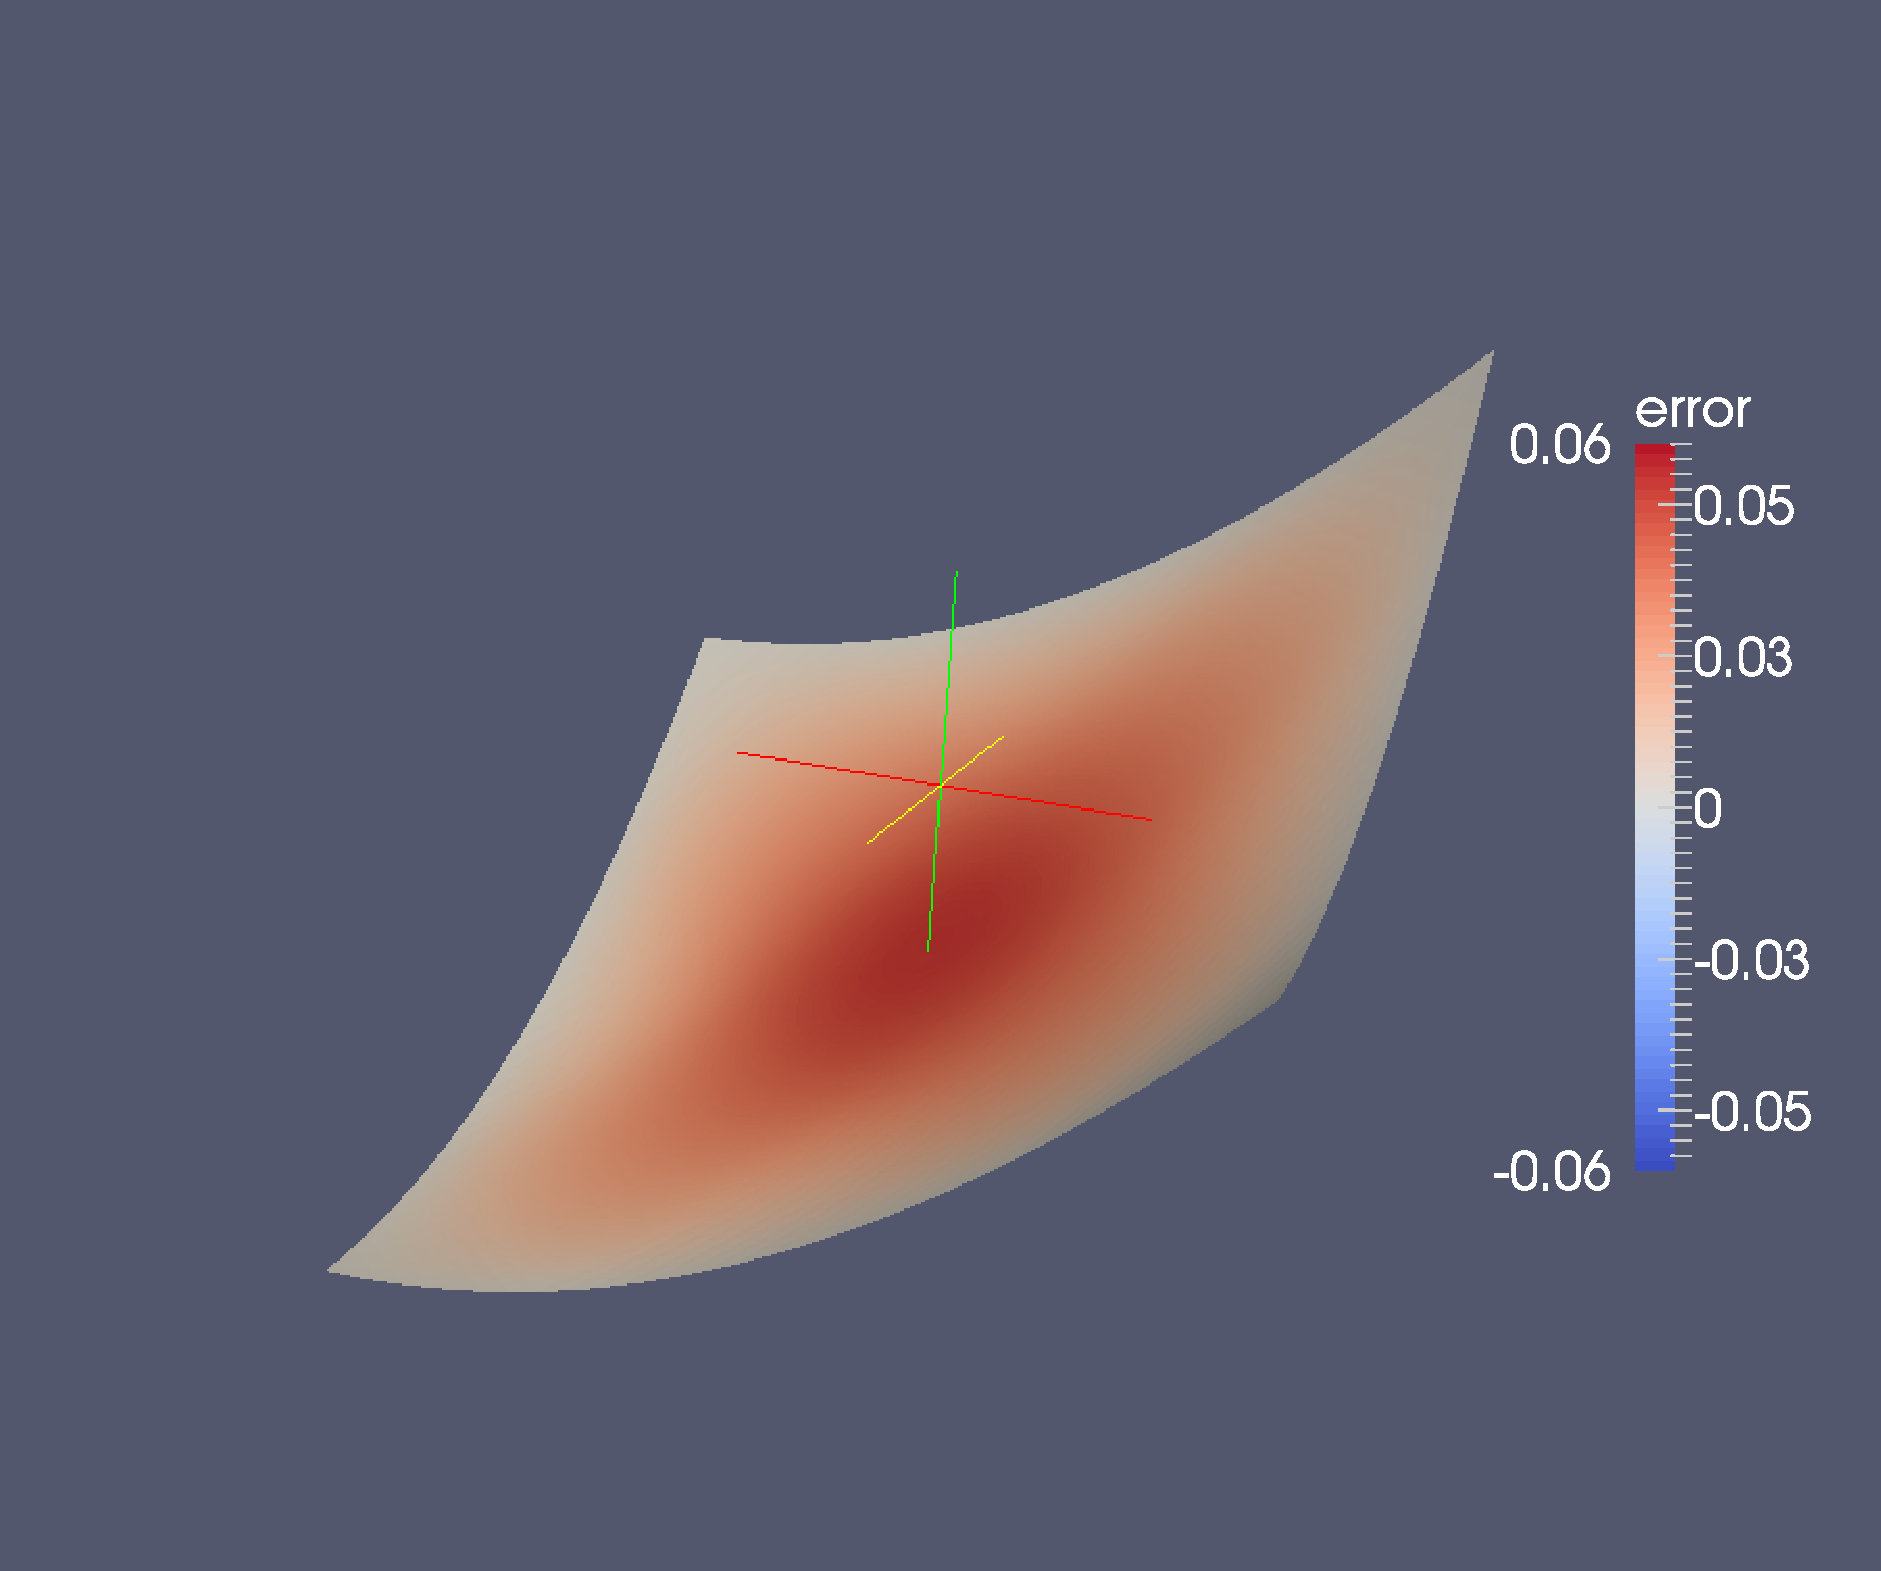
\includegraphics[width=1.\textwidth]{../Arbeit/plots/with_penalty_it22.pdf}
		\caption{Solution after 23 steps}
	\end{subfigure}
	~
	\begin{subfigure}[b]{.45\textwidth}
		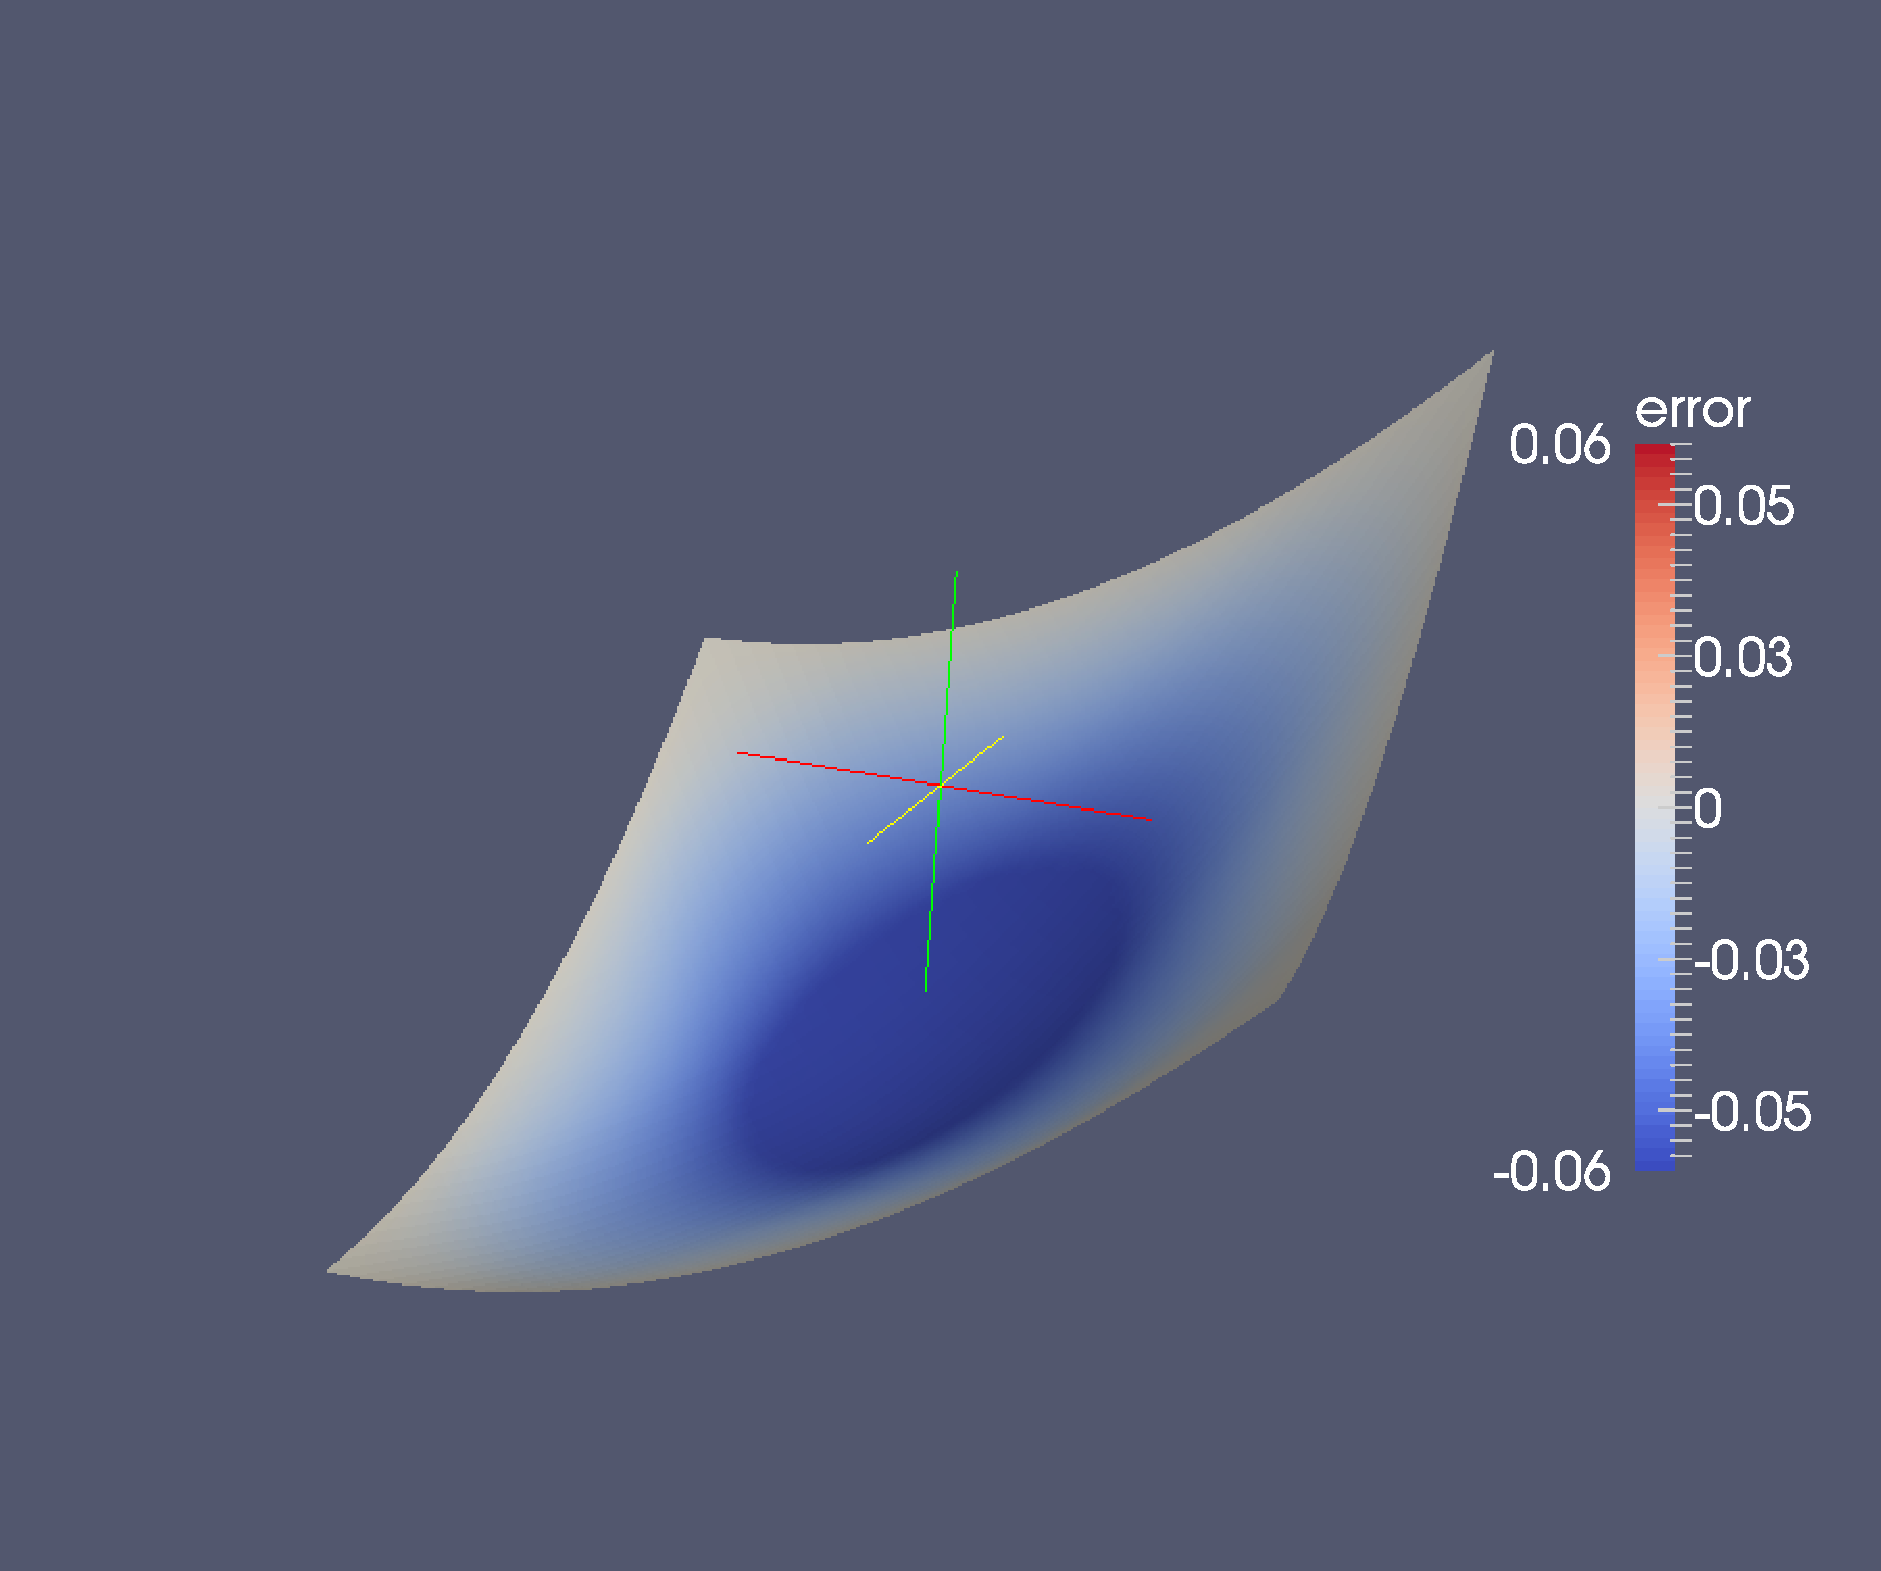
\includegraphics[width=1.\textwidth]{../Arbeit/plots/with_penalty_it23.pdf}
		\caption{Solution after 24 steps}
	\end{subfigure}
	\caption{The solution in two consecutive iterations}
	\end{figure}
\end{frame}

\begin{frame}{Damping of the Picard iteration}
	\begin{figure}[H]
		\centering
		\includegraphics[trim = 2cm 4cm 1cm 4cm, height = 0.6\textheight]{../Arbeit/plots/oscillation.pdf}
		\caption{Relative $L^2$ error on a grid with $h=\frac 1 4$ and gradient penalty}
		\label{fig: oscillation}
	\end{figure}
	\pause
	\vspace{-0.5cm}
	$\Rightarrow$ Convex combination $ \alpha u_h^{i+1} + (1- \alpha) u_h^i$ for $\alpha \in (0,1)$
\end{frame}


\begin{frame}{Well-posedness of SIPG formulation}
\begin{itemize}
	\item The ellipticity constant of the SIPG bilinear form is only positive for $\sigma > \sigma^*$. 
	\pause
	
	\item $\sigma^*$ depends on $1/\lambda(\cofHess u)$, where  $\lambda(A)$ denotes the smallest eigenvalue of $A$.
\end{itemize}
	\pause
	$\Rightarrow$ scale $\sigma$ by $\frac 1 {\lambda^*}$ where $\lambda^*$ is an approximation of the smallest eigenvalue.\pause We choose
	
	\begin{block}{Approximation of $\lambda$}
	\[
		\lambda^* = \min_{q \in Q} \lambda(\cofHess {u_h(q)}),
	\]
	where $Q$ are the quadrature points.
	\end{block} 
	
\end{frame}

\begin{frame}{Well-posedness of SIPG formulation}
\begin{itemize}
	\item For ellipticity of the SIPG bilinear form we need $\mycof {D^2_h u_h}$ to be positive definite.\\
	\pause
	\item Bound ellipticity constant from below with a constant
\end{itemize}
	\pause
	\begin{block}{Modified Cofactor Matrix}
		\[ 
			\mycofMod {D^2_h u_h} = \begin{cases}
			\mycof {D^2_h u_h} & \lambda \geq \varepsilon	\\
			\mycof {D^2_h u_h}+ (-\lambda+\varepsilon) Id%\begin{pmatrix} -\lambda+\varepsilon & 0 \\ 0 & -\lambda+\varepsilon \end{pmatrix} 
			& else
			\end{cases}
		\]
	\end{block}
	\pause
	\[
		\mycof {D^2_h u_h} \text{ pos. def.} \Leftrightarrow \hess u \text{ pos. def.} \pause \Leftrightarrow u_h \text{ is convex}
	\]
	
	
\end{frame}



\begin{frame}{Convexification of intermediate solutions}
\begin{itemize}
	\item \MA equation in general does not posses a unique solution
	\item often (unique) convex solution required
\end{itemize} 
\pause
	$\Rightarrow$ convexify the solution after every step
\begin{itemize}
\pause
	\item connection between convexity and B\'ezier polynomials
	\item convexification is not simple
	\item discussion in numerical results
\end{itemize} 
\end{frame}

%\begin{frame}{Convexification Approach of Schumaker and Speleers{, \cite{SS2014}}}
%	Given the solution of the generalised Poisson problem $u^{gp}_h$ we seek for a convex spline minimising the error at the B\'ezier control points, i.e. 
%\begin{block}{Quadratic Program for Convexification}
%Find the B\'ezier coefficients $c$ minimising
%	\begin{align*}
%			\lVert A c - b \rVert_2, \qquad \text{ such that } Cc \geq 0. %\label{eq: convex lsq}
%	\end{align*}
%\end{block}
%\begin{itemize}
%	\item $A$ is the matrix evaluating the piecewise polynomial at the B\'ezier control points
%	\item $b$ are the function values of $u^{gp}_h$ at the B\'ezier control points
%	\item  $C$ is the matrix containing the conditions ensuring convexity on the whole domain
%\end{itemize}
%
%\end{frame}


%\subsection{Algorithm for the Picard Iteration}

\begin{frame}
\begin{algorithm}[H]
\begin{algorithmic}
\Require triangulation \triang, desired mesh width $H$, maximal number of intermediate steps $i_{max}$
\State $u_{0}\gets $ solution of  $
	\triangle u = \sqrt{2f} \text{ in } \Omega $ with $
	u = g \text{ on }\partial \Omega$ %\Comment initialisation
\While {$h < H$}
	\For {$i$ from 1 to $i_{max}$}
		\State $\sigma \gets \sigma /\lambda(\hess{u_h^{i-1}}) $
		\State $u_i \gets$ sol of generalised Poisson problem w. modified cofactor matrix
		\State (convexify)
		\State $u_i \gets \alpha u_{i-1} + (1-\alpha)u_i $ \Comment convex combination
	\EndFor
	\State $h, \triang, u_{0} \gets h/2, \triangFine, u_{i_{max}}$
\EndWhile
\end{algorithmic}
\caption{Picard Iteration Algorithm to Solve the MA Equation}
\label{alg: final}
\end{algorithm}
\end{frame}


\section{Numerical Results}

\subsection{Implementation}
\begin{frame}{Implementation}
	\begin{itemize}
		\item implemented in C++
		\item linear system solved directly by a cholesky decomposition
		\item convexification via a quadratic program (c.f. {\cite{SS2014}}) solved by the library IPOPT
		\item 15 steps on each grid before refinement
		\item uniform standard grid refinement
	\end{itemize}
\end{frame}

\subsection{Results with Convexification}
\begin{frame}{Smooth test problem}
\vspace{-0.5cm}
\[
	u=\exp( \lVert x \rVert_2^2  /2) 
	\text { and } 
	f = (1 + \lVert x \rVert_2^2) \exp( \lVert x \rVert^2).
\]
\vspace{-0.75cm}
\begin{figure}[H]
\centering
	\includegraphics[height=0.75\textheight]{MA1_convexify_cropped.pdf}
%	\caption{$L^2$ errors for Test \ref{test smooth} and additional convexification}
\end{figure}
\end{frame}

\begin{frame}{Impact of convexifaction}
Comparison of $L^2$ errors before and after convexification
\vspace{-0.75cm}
\begin{figure}[H]
	\centering
	\includegraphics[height=0.95\textheight]{../Arbeit/plots/MA1_convexComp.pdf}
\end{figure}
\end{frame}

\subsection{Results without Convexification}
\begin{frame}{Smooth test problem without convexification}
%\end{block}
\vspace{-0.75cm}
	\begin{figure}[H]
	\centering
	\includegraphics[ %trim = 3cm 4cm 0cm 2cm,
	width=\textwidth]{../Arbeit/plots/MA1.pdf}
%		\caption{$L^2$ error with grad penalty}
	\end{figure}
\end{frame}

\begin{frame}{Penalty parameter $\sigma^G$}
$L^2$ errors for different choices of $\sigma^G$
\vspace{-0.75cm}
\begin{figure}[H]
	\centering
	\includegraphics[height=0.95\textheight]{../Arbeit/plots/MA1_deg2_sigma.pdf}\end{figure}
\end{frame}

\begin{frame}{Convex combination with parameter $\alpha$}
$L^2$ errors for different choices of $\alpha$
\vspace{-0.75cm}
\begin{figure}[H]
	\centering
	\includegraphics[height=0.95\textheight]{../Arbeit/plots/MA1_deg2_alpha.pdf}\end{figure}
\end{frame}

\begin{frame}{$C^1$ test problem}
\vspace{-0.5cm}
\[
	u=\frac 1 2 \left( \max 0 {\lVert x - x_0 \rVert_2-0.2 }  \right)^2 
	\text { and } 
	f = \max 0 {1-\frac {0.2} {\lVert x - x_0 \rVert_2} }.
\]
\vspace{-0.75cm}
\begin{figure}[H]
\centering
	\includegraphics[height=0.85\textheight]{../Arbeit/plots/MA2.pdf}
%	\caption{$L^2$ errors for Test \ref{test smooth} and additional convexification}
\end{figure}
\end{frame}

\begin{frame}{Singular test problem}
\vspace{-0.5cm}
\[
	u = - \sqrt{ 2-  \lVert x \rVert_2^2}
	\text { and } 
	f = 2\left( 2-  \lVert x \rVert_2^2 \right)^{-2}
\]
\vspace{-0.75cm}
\begin{figure}[H]
\centering
	\includegraphics[height=0.85\textheight]{../Arbeit/plots/MA3.pdf}
%	\caption{$L^2$ errors for Test \ref{test smooth} and additional convexification}
\end{figure}
\end{frame}


\section{Conclusion and Perspective}

\begin{frame}{Conclusion}
	\begin{itemize}
		\item reviewed current DG methods
		\item derived a new DG method using Picard linearisation
		\item explored several improvements of the Picard DG method
		\item the Picard type iteration converges on coarse grids, but is unstable on finer grids
		\item current DG methods are applicable for problems with smooth solutions, but have problems or even fail on singular problems
	\end{itemize}
\end{frame}

%\subsection{Conclusion}
	
\begin{frame}{Perspective}
	\begin{itemize}
		\item investigate if decoupled PDE has more solutions than the solution $v=w$
		\item implemented convexification not useful, may only convexify on finer grids
		\item analysis of the impact of the gradient penalty term
		\item apply theory developed for Picard linearisations of convection terms
		\item extension to right-hand sides depending on $u$ and $\nabla u$ and more complicated left-hand sides
		\item three-dimensional case
	\end{itemize}
\end{frame}


\begin{frame}[allowframebreaks]{References}
\putbib[../Arbeit/my_additional_bibliography.bib]
\end{frame}
\end{bibunit}

%\begin{bibunit}[plain]

%\section*{DG Methods}
%
%\begin{frame}
%Naive Ansatz:
%\begin{align*}
%	\myIntX {\Omega} {\mydet {D^2 u} v} = \myIntX \Omega {fv} \qquad \text{ for all test functions } v. %\label{eq: naiv ansatz}
%\end{align*}
%\begin{itemize}
%	\item does not work for elements not in $C^1(\Omega)$
%\end{itemize}
%
%\begin{figure}[H]
%			\begin{center}
		\usetikzlibrary{matrix}

\begin{tikzpicture}[scale =2]
  \matrix (m) [matrix of math nodes,row sep=3em,column sep=4em,minimum width=2em]
  {
     F[u]=0 & F_h[u] =0 \\
     L_u(w) =0 & L_{u,h}(w_h)=0 \\};
  \path[-stealth]
    (m-1-1) edge node [left] {linearise} (m-2-1)
            edge node [above] {discretise} (m-1-2)
    (m-2-1.east|-m-2-2) edge node [below] {discretise} (m-2-2)
    (m-1-2) edge node [right] {linearise} (m-2-2);
\end{tikzpicture}
		\end{center}

%	\caption{Diagram about the relation between weak and strong linear operators. The diagram is taken from \cite[Fig 2.2]{FGN2013}}
%%		\label{fig: fe diagram}	
%	\end{figure}
%\end{frame}
%
%\subsection*{A $C^0$ Penalty Method }
%\begin{frame}{A $C^0$ penalty method dev. by Brenner et al.}
%\quoting {However, this naive method does not work either in practice or analysis, as the linearization of the  discrete problem is not consistent with the linearization of the continuous problem.\cite{BGN+2011}} 
%\vspace{1cm}
%\pause
%
%In \cite{BGN+2011} Brenner et alt. develop a method for $C^0$ elements
%
%They add terms to the \quoting{naive ansatz} such that 
%\begin{align*}
%	\bilin {F (u+w)} v = \bilin {L_{u,h} w} v + \bilin {Rw} v,
%\end{align*}
%where $L_{u,h}$ is a stable and consistent discretisation of $L_u$.
%
%\end{frame}
%
%%\begin{frame}
%%Let $V_h$ be ...
%%\begin{block}{A $C^0$ penalty method for the MA problem }
%%Find $u_h \in V_h$ such that
%%\begin{align*}
%%	&\myIntX {\Omega} {\left(f-\mydet {D^2_h u_h}\right) v_h} 
%%	+ \sum_{e \in \edgesi} \myIntS e { \jump {\average{\mycof{D^2 u_h} } \nabla u_h} v_h} \\
%%	&- \sum_{e \in \edgesb} \myIntS e { \jump{ \average{\mycof{D^2 u_h} } \nabla v_h} (u_h -g)} \\
%%	&+ \sigma  \sum_{e \in \edgesb} \frac 1 {h_e} \myIntS e { (u_h -g)} \; = 0 \qquad \forall v_h \in V_h %\label{eq: brenner method}
%%\end{align*}
%%\end{block}
%%\end{frame}
%
%\subsection*{A Finite Element Method based on a Discrete Hessian}
%
%\def \boxContent {	The discrete Hessian $D_{DH}^2 u$ of $u$ is the unique function which satisfy for all $B \in \Sigma_h=[\mathcal{P}_h^k]^{d \times d}$
%		\begin{align*}
%			\myIntX  \Omega { (D_{DH}^2 u : B) }
%			= \myIntX  \Omega { D^2_h u: B}
%				 -\sum_{ e \in \edgesi} \myIntS e {  \jump {\average B \nabla u }}. %\label{eq: discrete hessian}
%		\end{align*}}
%
%\begin{frame}{A FEM based on a Discrete Hessian dev. by Neilan}
%The Hessian fulfils for all $B \in [H^1(\Omega)]^{d \times d}$
%	\begin{align}
%		\myIntX  \Omega { (D^2 u : B)} = 
%			- \myIntX  \Omega { \left(\nabla \cdot B\right) \cdot \nabla u} 
%			+ \myIntS {\partial \Omega}  {B \nabla u \; \mathbf {n}}, \label{eq: part int hessian}
%	\end{align}
%	\onslide<2->{ the piecewise Hessian in general not.}
%\begin{overlayarea}{\textwidth}{0.7\textheight}
%	\only<3>{
%		\vspace{1cm}
%		Idea by Lakkis and Pryer \cite{LP2011} and generalised by Neilan \cite{Neilan2014}: \\
%		Replace Hessian $D^2 u$ by a discrete version $D_{DH}^2 u$ which fulfils \eqref{eq: part int hessian}.		
%		Find $u_h$ such that 
%		\[
%			\myIntX  \Omega { \left(\mydet{D_{DH}^2 u_h} - f \right) v_h} = 0 \qquad \text{ for all test functions } v_h
%		\]
%		
%		
%	}
%%	\onslide<4->
%%	{
%%	\begin{block}{Definition of Discrete Hessian}
%%		\boxContent
%%	\end{block}
%%	}
%%	
%%	\onslide<5-> {Note that in general the discrete Hessian is not symmetric.}
%	\end{overlayarea}
%\end{frame}
%
%%\begin{frame}
%%\begin{block}{A FE Method based on a Discrete Hessian}
%%Find $u_h \in V_h$ such that
%%\begin{align*}
%%		\myIntX  \Omega { \left(\mydet{D_{DH}^2 u_h} - f \right) v_h} = 0 \qquad \forall v_h \in V_h, %\label{eq: neilan eq1}
%%\end{align*}
%%where $D_{DH}^2 u_h$ satisfies for all $B_h \in \Sigma_h$
%%	\begin{align*}
%%		\myIntX  \Omega { (D_{DH}^2 u_h : B_h) }
%%		= \myIntX  \Omega { D^2_h u_h: B_h}
%%			 -\sum_{ e \in \edgesi} \myIntS e {  \jump {\average {B_h} \nabla u_h }}. %\tag{\ref{eq: discrete hessian}}
%%	\end{align*}
%%\end{block}
%%\end{frame}
%%
%%\begin{frame}
%%Special case for polynomial degree $k=1$
%%
%%\begin{block}{A FE Method based on a Discrete Hessian}
%%Find $u_h$ in $V_h$ such that for all $v \in V_h$
%%\begin{align*}
%%		\myIntX  \Omega { \left(\mydet{D_{DH}^2 u_h} - f \right) v_h}+ \textcolor{red}{\sum_{e \in \edgesi} \sigma |e |\myIntS e {\jump{ \nabla u} \jump {\nabla v}}} = 0, %\label{eq: neilan eq1}
%%\end{align*}
%%where $D_{DH}^2 u_h$ satisfies for all $B_h \in \Sigma_h$
%%	\begin{align*}
%%		\myIntX  \Omega { (D_{DH}^2 u_h : B_h) }
%%		= \myIntX  \Omega { D^2_h u_h: B_h}
%%			 -\sum_{ e \in \edgesi} \myIntS e {  \jump {\average {B_h} \nabla u_h }}. %\tag{\ref{eq: discrete hessian}}
%%	\end{align*}
%%\end{block}
%%\end{frame}
%
%
%\subsection*{Numerical Results}
%\begin{frame}{Implementation}
%	\begin{itemize}
%		\item implemented with finite element tool FEniCS
%%	  \item nested iteration with  initial guess $\triangle u = - \sqrt{2f}$
%		\item uniform standard grid refinement
%		\item nonlinear system solved PETSc with FEniCS default configuration: a Newton based nonlinear solver using a basic line search, arising linear systems are solved by a $LU$ decomposition.
%		\item absolute tolerance is adjusted to $1e-8$ and number of maximum iteration restricted to 100
%	\end{itemize}
%\end{frame}
%
%\begin{frame}{Smooth test case for the $C^0$ penalty method}
%%\begin{block}
%Smooth Test Problem:
%\[
%	u=\exp( \lVert x \rVert_2^2  /2) 
%	\text { and } 
%	f = (1 + \lVert x \rVert_2^2) \exp( \lVert x \rVert^2).
%\]
%%\end{block}
%\vspace{-1cm}
%\begin{figure}[H]
%\centering
%	\includegraphics[width=0.95\textwidth]{../Arbeit/plots/MA1_Brenner_l2.pdf}
%%	\caption{$L^2$ errors for the smooth test case}
%\end{figure}
%\end{frame}
%
%%\newcommand{\readData}[2]{
%%	\pgfplotstableread{../Arbeit/data/#1_l2errornorm} #2
%%	
%%	\pgfplotstablecreatecol[copy column from table={../Arbeit/data/#1_h1errornorm}{h1error}] {h1error} #2
%%	
%%	\pgfplotstablecreatecol[copy column from table={../Arbeit/data/#1_newtonSteps}{steps}] {N} #2
%%}
%
%%\readData{MA3_Brenner_deg2}{\MAThreeBrennerTwo}
%%\readData{MA3_Brenner_deg3}{\MAThreeBrennerThree}
%
%%\begin{frame}
%%
%%\begin{table}[h]
%%\centering
%%	\begin{subtable}[b]{0.45\textwidth}
%%		\centering
%%		\pgfplotstabletypeset[columns={iterations, l2error, h1error,N},
%%				    every row 0 column 0/.style={set content=init},
%%		]\MAThreeBrennerTwo
%%    	\caption{Error for $k=2$}
%%    \end{subtable}
%%   ~
%%	\begin{subtable}[b]{0.45\textwidth}
%%		\centering
%%		\pgfplotstabletypeset[columns={iterations, l2error, h1error,N},
%%				    every row 0 column 0/.style={set content=init},
%%				    every row 0 column 0/.style={set content=init},
%%				    every row 3 column 1/.style={set content=-},
%%				    every row 3 column 2/.style={set content=-},
%%				    every row 3 column 3/.style={set content=-},
%%				    every row 4 column 1/.style={set content=-},
%%				    every row 4 column 2/.style={set content=-},
%%				    every row 4 column 3/.style={set content=-},
%%		]\MAThreeBrennerThree
%%    	\caption{Error for $k=3$}
%%    \end{subtable}	\caption{Errors for Test \ref{test singularity}}
%%	\label{tab: l2 errors test 3 Brenner}
%%\end{table}
%%\end{frame}
%
%\subsection*{A FE Method based on the Discrete Hessian}
%
%\begin{frame} %{Smooth Test Case}
%Smooth Test Problem:
%\[
%	u=\exp( \lVert x \rVert_2^2  /2) 
%	\text { and } 
%	f = (1 + \lVert x \rVert_2^2) \exp( \lVert x \rVert^2).
%\]
%\vspace{-1cm}
%\begin{figure}[H]
%\centering
%	\includegraphics[width=0.95\textwidth]{../Arbeit/plots/MA1_Neilan_l2.pdf}
%%	\caption{$L^2$ errors for Test \ref{test smooth}}
%\end{figure}
%\end{frame}
%
%\begin{frame}
%Smooth Problem solved with additional gradient penalty TODO right plot
%\vspace{-.75cm}
%	\begin{figure}[H]
%	\centering
%	\includegraphics[ %trim = 3cm 4cm 0cm 2cm,
%	width=\textwidth]{../Arbeit/plots/MA1_Neilan_l2.pdf}
%%		\caption{$L^2$ error with grad penalty}
%	\end{figure}
%\end{frame}
%
%\begin{frame}
%Smooth Problem solved with additional gradient penalty TODO right plot
%\vspace{-.75cm}
%	\begin{figure}[H]
%	\centering
%	\includegraphics[ %trim = 3cm 4cm 0cm 2cm,
%	width=\textwidth]{../Arbeit/plots/MA1_Neilan_h1.pdf}
%%		\caption{$L^2$ error with grad penalty}
%	\end{figure}
%\end{frame}
%
%\begin{frame}{Conclusion}
%\begin{itemize}
%		\item the $C^0$ penalty method developed by Brenner et al. yields good results for smooth cases, but fails in non-smooth cases
%		\item the method based on a discrete Hessian improved by Neilan converges in smooth cases as well as in non-smooth tests
%		\item Neilan's method requires a lot of degrees of freedom
%		
%\end{itemize}
%\end{frame}
%
%\begin{frame}[allowframebreaks]{References}
%\putbib[../Arbeit/my_additional_bibliography.bib]
%\end{frame}
%\end{bibunit}
%
\end{document}